\documentclass[fleqn]{article}
\oddsidemargin 0.0in
\textwidth 6.0in
\thispagestyle{empty}
\usepackage{import}
\usepackage{amsmath}
\usepackage{graphicx}
\usepackage{flexisym}
\usepackage{amssymb}
\usepackage{bigints} 
\usepackage[english]{babel}
\usepackage[utf8x]{inputenc}
\usepackage{float}
\usepackage[colorinlistoftodos]{todonotes}

\definecolor{hwColor}{HTML}{AD53BA}

\begin{document}

  \begin{titlepage}

    \newcommand{\HRule}{\rule{\linewidth}{0.5mm}}

    \center


    \textsc{\LARGE Arizona State University}\\[1.5cm]

    \textsc{\LARGE Advanced Calculus I }\\[1.5cm]


    \begin{figure}
      
\includegraphics[width=\linewidth]{asu.png}
    \end{figure}


    \HRule \\[0.4cm]
    { \huge \bfseries Homework One }\\[0.4cm] 
    \HRule \\[1.5cm]

    \textbf{Behnam Amiri}

    \bigbreak

    \textbf{Prof: Sergei Suslov}

    \bigbreak


    \textbf{{\large \today}\\[2cm]}

    \vfill

  \end{titlepage}

  \begin{enumerate}
    \item Simplify each expression, where possible, in the following list. Give the
    principal value of inverse trigonometric functions, where applicable. If no
    simplification is possible, then so state.

    \begin{itemize}
      \item $ln (x^3)+ln (x^4)$.

        \textcolor{hwColor}{
          \\
          $
            ln (x^3)+ln (x^4)=ln(x^3 \times x^7)=ln(x^{10})
            \\
            \\
            \therefore ~~~~ ln (x^3)+ln (x^4)=10 ln(x) ~~~~ \checkmark
            \\
          $
        }

      \item $e^{\dfrac{ln (x)}{2}}$.

        \textcolor{hwColor}{
          \\
          $
            e^{\dfrac{ln (x)}{2}}=e^{\dfrac{1}{2} ln(x)}
            e^{ln(x)^{\dfrac{1}{2}}}=x^{\dfrac{1}{2}}
            \\
            \\
            \\
            \therefore ~~~~ e^{\dfrac{ln (x)}{2}}=\sqrt{x} ~~~~ \checkmark
          $
        }

      \item $e^{ln 7-ln 8}$.

        \textcolor{hwColor}{
          \\
          $
            e^{ln 7-ln 8}=e^{ln\left(\dfrac{7}{8}\right)}
            \\
            \\
            \\
            \therefore ~~~~ e^{ln 7-ln 8}=\dfrac{7}{8} ~~~~ \checkmark
            \\
          $
        }

      \item $e^0$.

        \textcolor{hwColor}{
          \\
          $
            e^0=1
            \\
          $
        }

      \item $cos^{2}(x)-1$.

        \textcolor{hwColor}{
          \\
          $
            sin^2(x)+cos^2(x)=1 \Longrightarrow 1-cos^2(x)=sin^2(x)
            \\
            \\
            \\
            \therefore ~~~~ cos^{2}(x)-1=-sin^2(x) ~~~~ \checkmark
            \\
          $ 
        }

      \item $sin(-x)$.

        \textcolor{hwColor}{
          \\
          $
            sin(-x)=-sin(x)
            \\
          $
        }

      \item $tan(\dfrac{\pi}{4})$.

        \textcolor{hwColor}{
          \\
          $
            tan(\dfrac{\pi}{4})
            =\dfrac{sin(\dfrac{\pi}{4})}{cos(\dfrac{\pi}{4})}
            =\dfrac{\dfrac{\sqrt{2}}{2}}{\dfrac{\sqrt{2}}{2}}
            \\
            \\
            \\
            \therefore ~~~~ tan(\dfrac{\pi}{4})=1 ~~~~ \checkmark
            \\
          $
        }

      \item $Arctan(1)$.

        \textcolor{hwColor}{
          \\
          Based on the definition of $Arctan$, we know that $tan(\theta)=1$, hence $Arctan(1)=\theta$. 
          The only values of $\theta$ that make $tan(\theta)=1$ are $\dfrac{\pi}{4}$ and $\dfrac{5 \pi}{4}$.
          Note that the range of $Arctan$ is $\left(-\dfrac{\pi}{2}, +\dfrac{\pi}{2}\right)$, therefore
          $\dfrac{\pi}{4}$ is the correct answer.
          \\
        }

    \end{itemize}


    \item Solve for $x$ where possible
    \begin{itemize}
      \item $ln(2x+2)=3t$.

        \textcolor{hwColor}{
          \\
          $
            ln(2x+2)=3t \Longrightarrow e^{3t}=2x+2
            \\
            \\
            \\
            \therefore ~~~~ x=\dfrac{e^{3t}-2}{2} ~~~~ \checkmark
            \\
          $
        }

      \item $x^2+4x+3=0$.

        \textcolor{hwColor}{
          \\
          $
            x^2+4x+3=0 \Longrightarrow (x+1)(x+3)=0 \Longrightarrow \begin{cases}
              x+1=0
              \\
              x+3=0
            \end{cases} \Longrightarrow \begin{cases}
              x=-1
              \\
              x=-3
            \end{cases} ~~~~ \checkmark
            \\
          $
        }

      \item $x^3+2x^2+x=0$.

        \textcolor{hwColor}{
          \\
          $
            x^3+2x^2+x=0 \Longrightarrow x \left(x^2+2x+1\right)=x(x+1)(x+1)=0
            \\
            \\
            \\
            \therefore ~~~~ \begin{cases}
              x=0
              \\
              x=-1
            \end{cases} ~~~~ \checkmark
          $
        }

      \item $Arctan (x)=1$.

        \textcolor{hwColor}{
          \\
          Based on the definition of $Arctan$, we know that $tan(\theta)=1$, hence $Arctan(1)=\theta$. 
          The only values of $\theta$ that make $tan(\theta)=1$ are $\dfrac{\pi}{4}$ and $\dfrac{5 \pi}{4}$.
          Note that the range of $Arctan$ is $\left(-\dfrac{\pi}{2}, +\dfrac{\pi}{2}\right)$, therefore
          $\dfrac{\pi}{4}$ is the correct answer.
        }

      \item $Arcsin (x)=\dfrac{\sqrt{2}}{2}$.

      \textcolor{hwColor}{
        \\
        We know that $sin(\dfrac{\pi}{4})=\dfrac{\sqrt{2}}{2}$ is the length of a right-angled triangle 
        with sides $\dfrac{\sqrt{2}}{2}, ~ \dfrac{\sqrt{2}}{2}$ and $1$ which has internal 
        angles $\dfrac{\pi}{4}, ~ \dfrac{\pi}{4}$ and $\dfrac{\pi}{2}$. Also we know that $\dfrac{\pi}{4}$ is
        in the required range for $Arcsin(x)$ is $\left[-\dfrac{\pi}{2}, +\dfrac{\pi}{2}\right]$.
        \\
        \\
        \\
        $
          \therefore ~~~~ Arcsin(\dfrac{\sqrt{2}}{2})=\dfrac{\pi}{4} ~~~~ \checkmark
          \\
        $ 
      }

    \end{itemize}

    \item Find the indicated derivative of each of the following expression.
    \begin{itemize}
      \item $\dfrac{d}{dt} \left(e^{-3t}\right)$.

        \textcolor{hwColor}{
          \\
          $
            \dfrac{d}{dt} \left(e^{-3t}\right)=e^{-3t} \times ln(e) \times \dfrac{d}{dt} \left(-3t\right)
            \\
            \\
            \\
            \therefore ~~~~ \dfrac{d}{dt} \left(e^{-3t}\right)=-3e^{-3t} ~~~~ \checkmark
            \\
          $
        }

      \item $\dfrac{d}{dt} \left(\dfrac{3}{t}\right)$.

        \textcolor{hwColor}{
          \\
          $
            \dfrac{d}{dt} \left(\dfrac{3}{t}\right)=\dfrac{(0 \times t)-(1 \times 3)}{t^2}
            \\
            \\
            \\
            \therefore ~~~~ \dfrac{d}{dt} \left(\dfrac{3}{t}\right)=-\dfrac{3}{t^2} ~~~~ \checkmark
            \\
          $
        }

      \item $\dfrac{d}{dx} \left[sin(5x)\right]$.

        \textcolor{hwColor}{
          \\
          $
            \dfrac{d}{dx} \left[sin(5x)\right]=cos(5x) \times \dfrac{d}{dx} \left(5x\right)
            \\
            \\
            \\
            \therefore ~~~~ \dfrac{d}{dx} \left[sin(5x)\right]=5cos(5x) ~~~~ \checkmark
            \\
          $
        }

      \item $\dfrac{d}{dx} \left[tan(x)\right]$.

        \textcolor{hwColor}{
          \\
          $
            \dfrac{d}{dx} \left[tan(x)\right]=\dfrac{d}{dx} \left[\dfrac{sin(x)}{cos(x)}\right]
            =\dfrac{cos(x).cos(x)-\left[-sin(x)\right]sin(x)}{cos^2(x)}
            =\dfrac{cos^2(x)+sin^2(x)}{cos^2(x)}
            \\
            \\
            \\
            \therefore ~~~~ \dfrac{d}{dx} \left[tan(x)\right]=\dfrac{1}{cos^2(x)}=sec^2(x) ~~~~ \checkmark
          $
        }

      \item $\dfrac{d}{dt} \left[t cos(t)\right]$.

        \textcolor{hwColor}{
          \\
          $
            \dfrac{d}{dt} \left[t cos(t)\right]=cos(t)+\left[-sin(t)t\right]
            \\
            \\
            \\
            \therefore ~~~~ \dfrac{d}{dt} \left[t cos(t)\right]=cos(t)-tsin(t) ~~~~ \checkmark
            \\
          $
        }

      \item $\dfrac{d}{dt} \left[ln(2t)\right]$.

        \textcolor{hwColor}{
          \\
          $
            \dfrac{d}{dt} \left[ln(2t)\right]=\dfrac{1}{2t} \dfrac{d}{dt} (2t)
            \\
            \\
            \\
            \therefore ~~~~ \dfrac{d}{dt} \left[ln(2t)\right]=\dfrac{1}{t} ~~~~ \checkmark
            \\
          $
        }

      \item $\dfrac{d}{dx} \left[\left(2x+4\right)^{10}\right]$.

        \textcolor{hwColor}{
          \\
          $
            \dfrac{d}{dx} \left[\left(2x+4\right)^{10}\right]=10(2)(2x+4)^9
            \\
            \\
            \\
            \therefore ~~~~ \dfrac{d}{dx} \left[\left(2x+4\right)^{10}\right]=20\left(2x+4\right)^9 ~~~~ \checkmark
            \\
          $
        }

      \item $\dfrac{d}{dx} \left(9x^8+\dfrac{1}{x^2}\right)$.

        \textcolor{hwColor}{
          \\
          $
            \dfrac{d}{dx} \left(9x^8+\dfrac{1}{x^2}\right)=72x^7+\dfrac{(0 \times x^2)-(2x \times 1)}{x^4}
            \\
            \\
            \\
            \therefore ~~~~ \dfrac{d}{dx} \left(9x^8+\dfrac{1}{x^2}\right)=72x^7-\dfrac{2}{x^3} ~~~~ \checkmark
            \\
          $
        }

      \item $\dfrac{d}{dx} \left(\dfrac{1}{\sqrt{2x+1}}\right)$.

        \textcolor{hwColor}{
          \\
          $
            \dfrac{d}{dx} \left(\dfrac{1}{\sqrt{2x+1}}\right)=\dfrac{(0 \times \sqrt{2x+1})-\dfrac{d}{dx} \left[\sqrt{2x+1}\right]}{\left(\sqrt{2x+1}\right)^2}
            =\dfrac{-\dfrac{1}{\sqrt{2x+1}}}{\left(\sqrt{2x+1}\right)^2}
            \\
            \\
            \\
            \therefore ~~~~ \dfrac{d}{dx} \left(\dfrac{1}{\sqrt{2x+1}}\right)=-\dfrac{1}{\left(2x+1\right)^{3/2}} ~~~~ \checkmark
            \\
          $
        }

      \item $\dfrac{d}{dt} \left(3t^2+1\right)^{\dfrac{3}{2}}$.

        \textcolor{hwColor}{
          \\
          $
            \dfrac{d}{dt} \left(3t^2+1\right)^{\dfrac{3}{2}}=\dfrac{3}{2} \left(6t\right) \left(3t^2+1\right)^{\dfrac{1}{2}}
            \\
            \\
            \\
            \therefore ~~~~ \dfrac{d}{dt} \left(3t^2+1\right)^{\dfrac{3}{2}}=9t \left(3t^2+1\right)^{\dfrac{1}{2}} ~~~~ \checkmark
            \\
          $
        }

      \item $\dfrac{d}{dt} \left(\dfrac{1}{\sqrt[3]{t+1}}\right)$.

        \textcolor{hwColor}{
          \\
          $
            \dfrac{d}{dt} \left(\dfrac{1}{\sqrt[3]{t+1}}\right)
            =\dfrac{d}{dt} \left(\dfrac{1}{(t+1)^{1/3}}\right)
            =\dfrac{d}{dt} \left[\left(t+1\right)^{-1/3}\right]
            =-\dfrac{1}{3} (1) \left(t+1\right)^{-4/3}
            \\
            \\
            \\
            \therefore ~~~~ \dfrac{d}{dt} \left(\dfrac{1}{\sqrt[3]{t+1}}\right)=-\dfrac{1}{3\left(t+1\right)^{4/3}} ~~~~ \checkmark
            \\
          $
        }

      \item $\dfrac{d}{dt} \left(2t+1\right)^{\dfrac{1}{4}}$.

        \textcolor{hwColor}{
          \\
          $
            \dfrac{d}{dt} \left(2t+1\right)^{\dfrac{1}{4}}=\dfrac{1}{4} (2) \left(2t+1\right)^{-\dfrac{3}{4}}
            \\
            \\
            \\
            \therefore ~~~~ \dfrac{d}{dt} \left(2t+1\right)^{\dfrac{1}{4}}=\dfrac{1}{2 \left(2t+1\right)^{3/4}} ~~~~ \checkmark
            \\
          $
        }

    \end{itemize}

    \item Evaluate each of the following limits. If the limit does not exist, then so
    state. Note that some limits may be $+\infty$ or $-\infty$; an infinite limit is not the
    same as a limit that does not exist. Give the principal value of the limits of
    inverse trigonometric functions, where applicable.
    \begin{itemize}
      \item $\lim\limits_{t \to \infty} e^{-t}$.

        \textcolor{hwColor}{
          \\
          \textbf{Option 1:}
          \\
          $
            \lim\limits_{t \to \infty} e^{-t}=\lim\limits_{t \to \infty} \dfrac{1}{e^t}=\dfrac{\lim\limits_{t \to \infty} 1}{\lim\limits_{t \to \infty} e^t}=\dfrac{1}{\infty}
            \\
            \\
            \\
            \therefore ~~~~ \lim\limits_{t \to \infty} e^{-t}=0 ~~~~ \checkmark 
          $
          \\
          \\
          \rule{15cm}{1pt}
          \\
          \\
          \textbf{Option 2:}
          \\
          $
            \lim\limits_{t \to \infty} e^{-t}
            =e^{\lim\limits_{t \to \infty} \left(-t\right)}
            =e^{-\lim\limits_{t \to \infty} t}
            =e^{-\infty}
            \\
            \\
            \\
            \therefore ~~~~ \lim\limits_{t \to \infty} e^{-t}=0 ~~~~ \checkmark
            \\
          $
          \\
          \\
          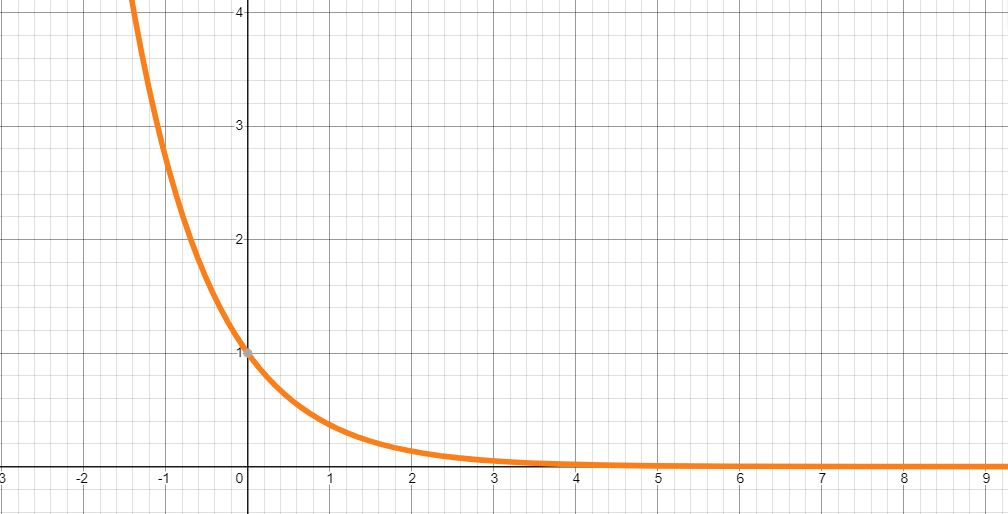
\includegraphics[width=10cm, height=6cm]{Twelve.JPG}
          \\
          \\
        }
      
      \item $\lim\limits_{x \to \infty} e^{2-x}$.

        \textcolor{hwColor}{
          \\
          $
            \lim\limits_{x \to \infty} e^{2-x}
            =\lim\limits_{x \to \infty} \left[e^2 e^{-x}\right]
            =e^2 \lim\limits_{x \to \infty} e^{-x}
            =e^2 \times 0
            \\
            \\
            \\
            \therefore ~~~~ \lim\limits_{x \to \infty} e^{2-x}=0 ~~~~ \checkmark
            \\
          $
          \\
          \\
          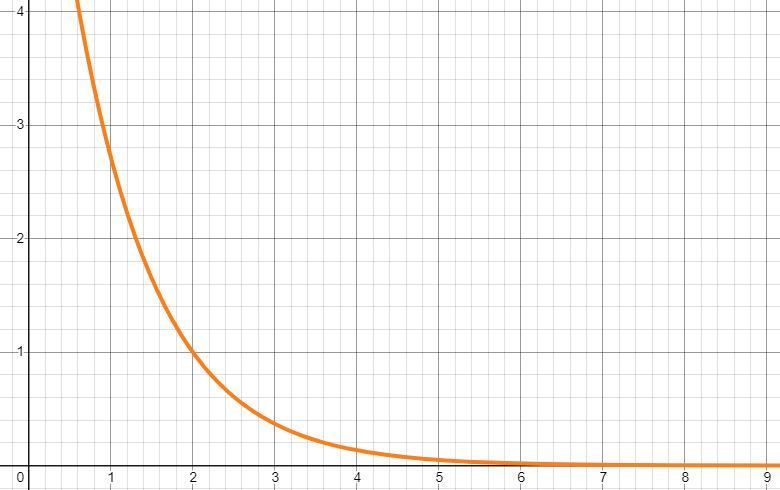
\includegraphics[width=10cm, height=6cm]{Eleven.JPG}
          \\
          \\
        }

      \item $\lim\limits_{x \to \infty} e^{\dfrac{1}{x}}$.
      
        \textcolor{hwColor}{
          \\
          $
            \lim\limits_{x \to \infty} e^{\dfrac{1}{x}}
            =e^{\lim\limits_{x \to \infty} \dfrac{1}{x}}
            =e^{\dfrac{\lim\limits_{x \to \infty} 1}{\lim\limits_{x \to \infty} x}}
            =e^{\dfrac{1}{\infty}}
            =e^0
            \\
            \\
            \\
            \therefore ~~~~ \lim\limits_{x \to \infty} e^{\dfrac{1}{x}}=1 ~~~~ \checkmark
            \\
          $
          \\
          \\
          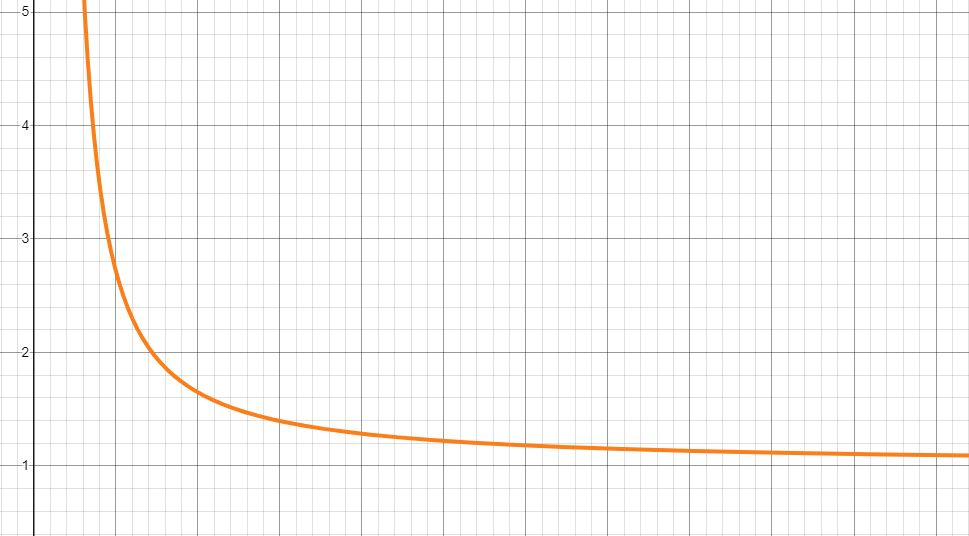
\includegraphics[width=10cm, height=6cm]{Ten.JPG}
          \\
          \\
        }

      \item $\lim\limits_{x \to 0} e^{-x}$. 

        \textcolor{hwColor}{
          \\
          $
            \lim\limits_{x \to 0} e^{-x}=e^{-0}
            \\
            \\
            \\
            \therefore ~~~~ \lim\limits_{x \to 0} e^{-x}=1 ~~~~ \checkmark
            \\
          $
          \\
          \\
          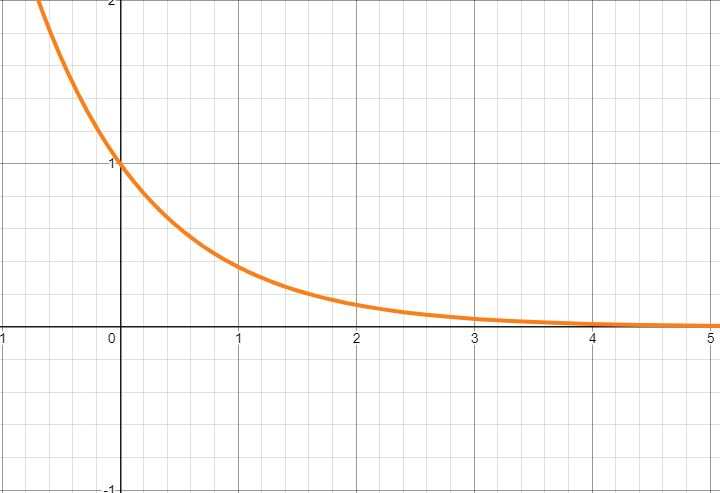
\includegraphics[width=10cm, height=6cm]{Nine.JPG}
          \\
          \\
        }

      \item $\lim\limits_{x \to 0} \left(x e^{-x}\right)$.

        \textcolor{hwColor}{
          \\
          $
            \lim\limits_{x \to 0} \left(x e^{-x}\right)=0 \times e^{-0}
            \\
            \\
            \\
            \therefore ~~~~ \lim\limits_{x \to 0} \left(x e^{-x}\right)=0  ~~~~ \checkmark
            \\
          $
          \\
          \\
          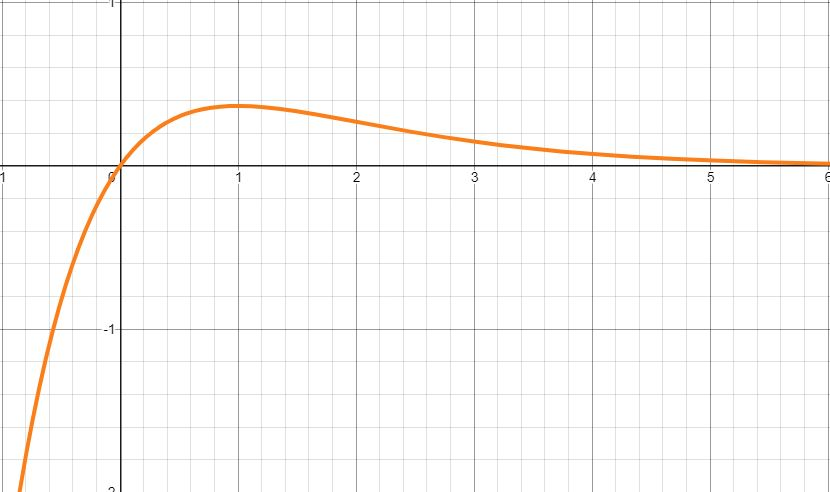
\includegraphics[width=10cm, height=6cm]{Eight.JPG}
          \\
          \\
        }
      
      \item $\lim\limits_{x \to 0} tan(x)$. 

        \textcolor{hwColor}{
          \\
          $
            \lim\limits_{x \to 0} tan(x)=\lim\limits_{x \to 0} \dfrac{sin(x)}{cos(x)}
            =\dfrac{\lim\limits_{x \to 0} sin(x)}{\lim\limits_{x \to 0} cos(x)}
            =\dfrac{sin(0)}{cos(0)}=\dfrac{0}{1}
            \\
            \\
            \\
            \therefore ~~~~ \lim\limits_{x \to 0} tan(x)=0 ~~~~ \checkmark
            \\
          $
          \\
          \\
          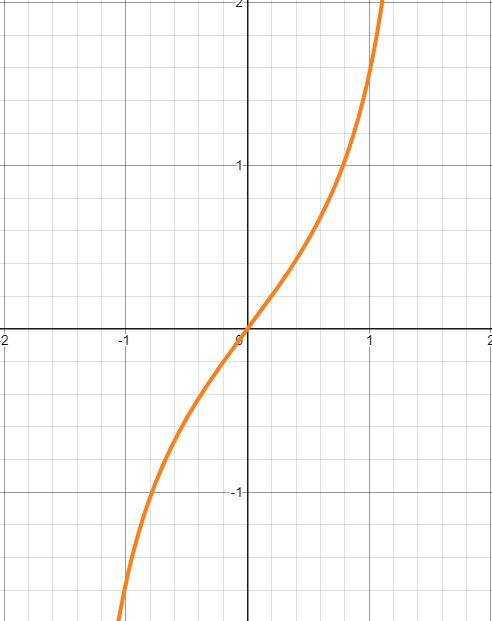
\includegraphics[width=10cm, height=6cm]{Seven.JPG}
          \\
          \\
        }

      \item $\lim\limits_{x \to 0} \dfrac{sin(x)}{x}$. 

        \textcolor{hwColor}{
          \\
          We can apply the l'Hopital's rule since $\dfrac{0}{0}$ is indeterminate. \\
          $
            \lim\limits_{x \to 0} \dfrac{sin(x)}{x}
            =\lim\limits_{x \to 0} \dfrac{\dfrac{d}{dx}\left[sin(x)\right]}{\dfrac{d}{dx}(x)}
            =\lim\limits_{x \to 0} \dfrac{cos(x)}{1}=\lim\limits_{x \to 0} cos(0)
            \\
            \\
            \\
            \therefore ~~~~ \lim\limits_{x \to 0} \dfrac{sin(x)}{x}=1 ~~~~ \checkmark
            \\
          $
          \\
          \\
          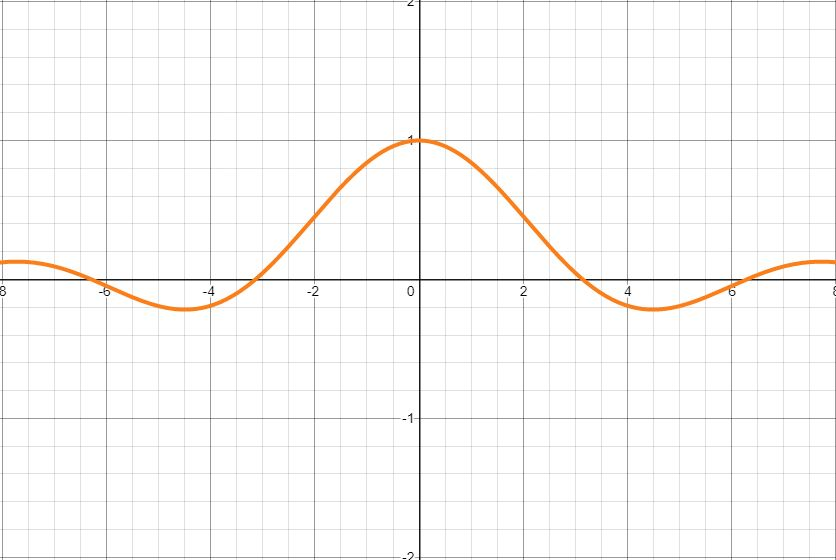
\includegraphics[width=10cm, height=6cm]{Six.JPG}
          \\
          \\
        }

      \item $\lim\limits_{x \to 0} \dfrac{cos(x)}{x}$. 

        \textcolor{hwColor}{
          \\
          We know that the Taylor series expansion of $cos(x)$ is 
          $
            \sum\limits_{n=0}^{\infty} (-1)^n \dfrac{x^{2n}}{(2n)!}
          $
          \\
          \\
          \textbf{Limit from right:}
          \\
          \\
          $
            \lim\limits_{x \to 0^+} \dfrac{cos(x)}{x}
            =\lim\limits_{x \to 0^+} \dfrac{1-\dfrac{x^2}{2!}+\dfrac{x^4}{4!}-\dfrac{x^6}{6!}+\dfrac{x^8}{8!}-...}{x}
            =\lim\limits_{x \to 0^+} \dfrac{1}{x}-\dfrac{x}{2}+\dfrac{x^3}{4!}-\dfrac{x^5}{6!}+...
            \\
            \\
          $
          When $x$ approaches to $0$, all the terms from the 2nd onwards become $0$. 
          Therefore, the only term left is the first term, which is $\lim\limits_{x \to 0^+} \dfrac{1}{x}$. This 
          leaves us with $+\infty$.
          \\
          \\
          $
            \therefore ~~~~ \lim\limits_{x \to 0^+} \dfrac{cos(x)}{x}=+\infty ~~~~ \checkmark
          $
          \\
          \\
          \rule{15cm}{2pt}
          \\
          \\
          \textbf{Limit from left:}
          \\
          \\
          $
            \lim\limits_{x \to 0^-} \dfrac{cos(x)}{x}
            =\lim\limits_{x \to 0^-} \dfrac{1-\dfrac{x^2}{2!}+\dfrac{x^4}{4!}-\dfrac{x^6}{6!}+\dfrac{x^8}{8!}-...}{x}
            =\lim\limits_{x \to 0^-} \dfrac{1}{x}-\dfrac{x}{2}+\dfrac{x^3}{4!}-\dfrac{x^5}{6!}+...
          $
          \\
          \\
          When $x$ approaches to $0$, all the terms from the 2nd onwards become $0$. 
          Therefore, the only term left is the first term, which is $\lim\limits_{x \to 0^+} \dfrac{1}{x}$. This 
          leaves us with $-\infty$.
          \\
          \\
          $
            \therefore ~~~~ \lim\limits_{x \to 0^-} \dfrac{cos(x)}{x}=-\infty ~~~~ \checkmark
          $
          \\
          \\
          \\
          Since $\lim\limits_{x \to 0^-} \dfrac{cos(x)}{x} \neq \lim\limits_{x \to 0^+} \dfrac{cos(x)}{x}$, 
          then $\lim\limits_{x \to 0} \dfrac{cos(x)}{x}$ \textbf{does not exist!}
          \\
          \\
          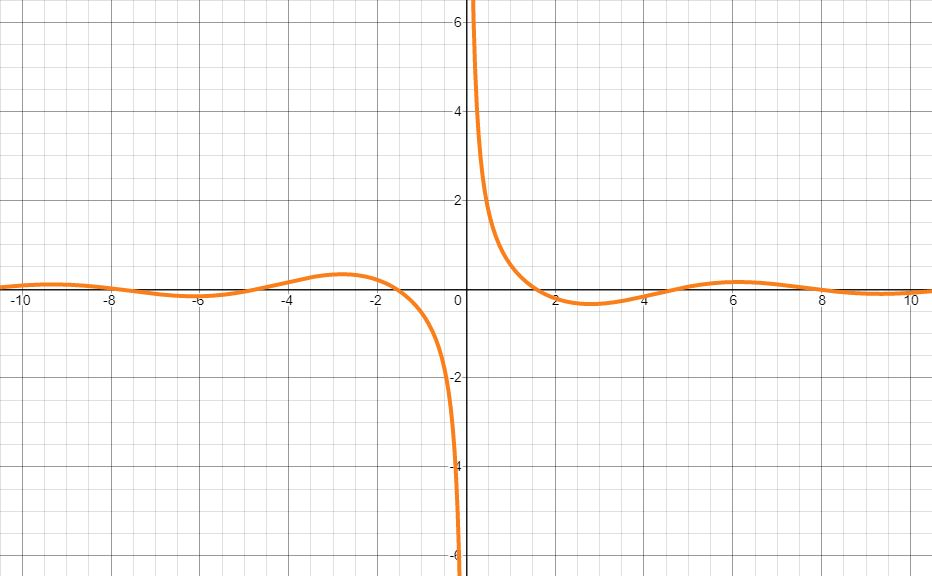
\includegraphics[width=10cm, height=6cm]{One.JPG}
          \\
          \\
        }

      \item $\lim\limits_{x \to 0} \dfrac{x}{3x^2+1}$.

        \textcolor{hwColor}{
          \\
          $
            \lim\limits_{x \to 0} \dfrac{x}{3x^2+1}=\dfrac{0}{3(0)^2+1}
            \\
            \\
            \\
            \therefore ~~~~ \lim\limits_{x \to 0} \dfrac{x}{3x^2+1}=0 ~~~~ \checkmark
            \\
          $
          \\
          \\
          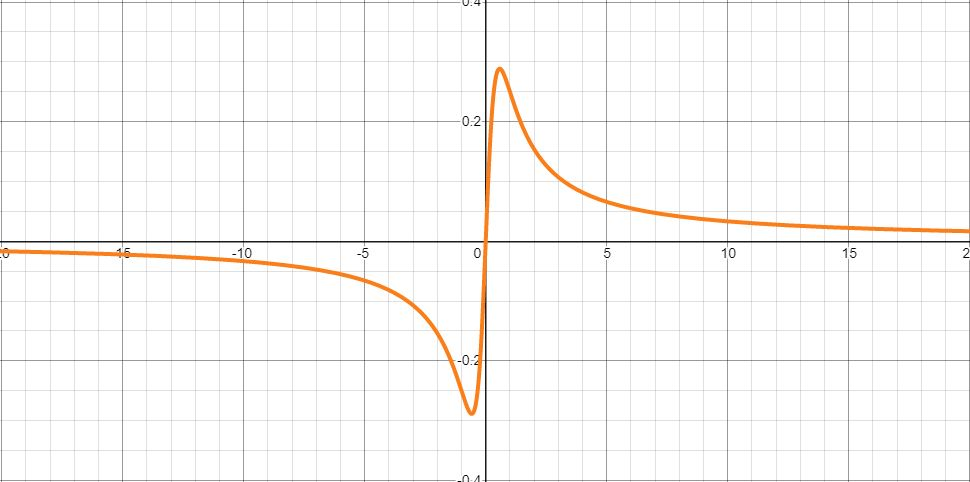
\includegraphics[width=10cm, height=6cm]{Two.JPG}
          \\
          \\
        }
      
      \item $\lim\limits_{x \to \infty} \dfrac{x}{3x^2+1}$. 

        \textcolor{hwColor}{
          \\
          $
            \lim\limits_{x \to \infty} \dfrac{x}{3x^2+1}
            =\lim\limits_{x \to \infty} \dfrac{\dfrac{1}{x}}{3+\dfrac{1}{x^2}}
            =\dfrac{\lim\limits_{x \to \infty} \left(\dfrac{1}{x}\right)}{\lim\limits_{x \to \infty} \left(3+\dfrac{1}{x^2}\right)}
            =\dfrac{0}{3}
            \\
            \\
            \\
            \therefore ~~~~ \lim\limits_{x \to \infty} \dfrac{x}{3x^2+1}=0 ~~~~ \checkmark
            \\
          $
          \\
          \\
          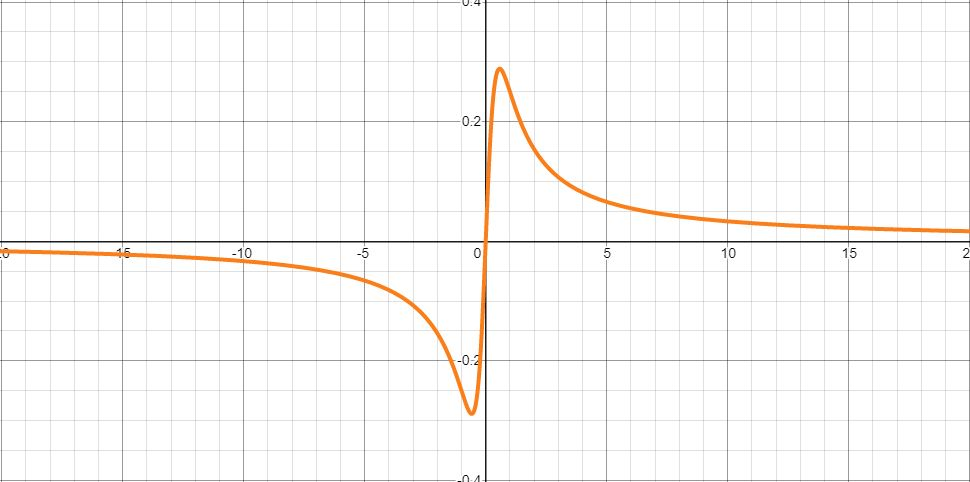
\includegraphics[width=10cm, height=6cm]{Two.JPG}
          \\
          \\
        }

      \item $\lim\limits_{x \to \infty} \dfrac{x^2+1}{x}$. 

        \textcolor{hwColor}{
          \\
          $
            \lim\limits_{x \to \infty} \dfrac{x^2+1}{x}
            =\lim\limits_{x \to \infty} \left(x+\dfrac{1}{x}\right)
            =\lim\limits_{x \to \infty} x+\lim\limits_{x \to \infty} \dfrac{1}{x}
            =\infty + 0
            \\
            \\
            \\
            \therefore ~~~~ \lim\limits_{x \to \infty} \dfrac{x^2+1}{x}=+\infty ~~~~ \checkmark
            \\
          $
          \\
          \\
          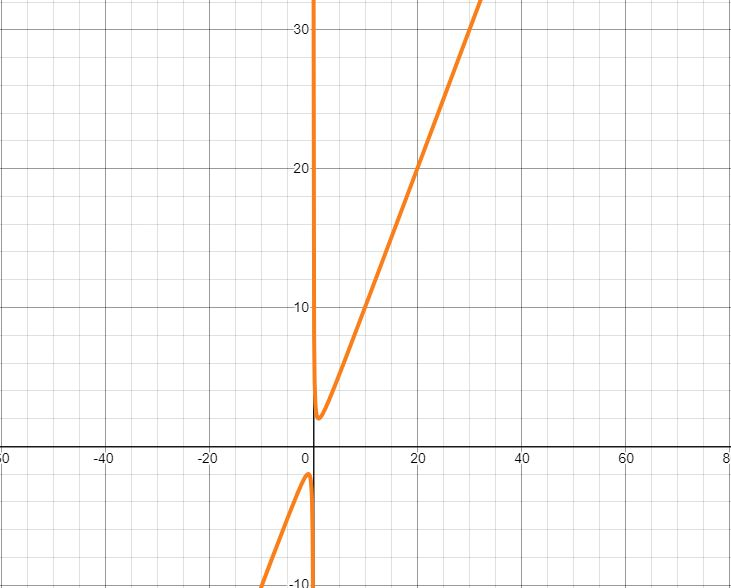
\includegraphics[width=10cm, height=6cm]{Five.JPG}
          \\
          \\
        }

      \item $\lim\limits_{x \to 0} \dfrac{x+1}{x-1}$. 

        \textcolor{hwColor}{
          \\
          $
            \lim\limits_{x \to 0} \dfrac{x+1}{x-1}=\dfrac{x+0}{0-1}
            \\
            \\
            \\
            \therefore ~~~~ \lim\limits_{x \to 0} \dfrac{x+1}{x-1}=-1 ~~~~ \checkmark
            \\
          $
          \\
          \\
          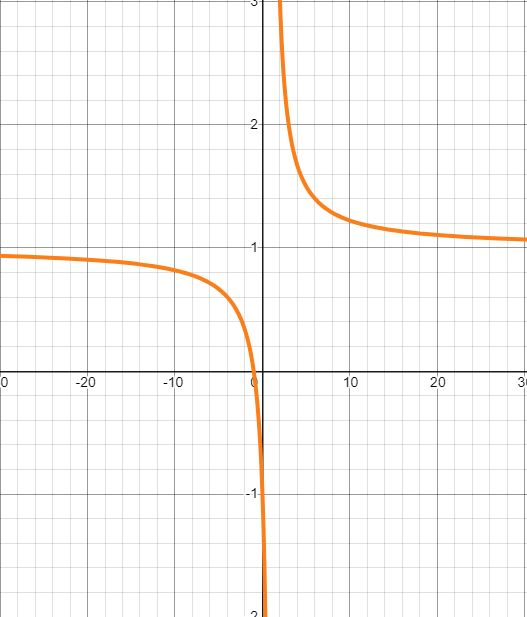
\includegraphics[width=10cm, height=6cm]{Four.JPG}
          \\
          \\
        }

      \item $\lim\limits_{x \to 1} \dfrac{x+1}{x-1}$.

        \textcolor{hwColor}{
          \\
          \textbf{Limit from left:}
          $
            \lim\limits_{x \to 1^-} \dfrac{x+1}{x-1}=-\infty
            \\
            \\
          $
          \\
          \textbf{Limit from right:}
          $
            \lim\limits_{x \to 1^+} \dfrac{x+1}{x-1}=+\infty
            \\
            \\
          $
          \\
          \\
          Since $\lim\limits_{x \to 1^-} \dfrac{x+1}{x-1} \neq \lim\limits_{x \to 1^+} \dfrac{x+1}{x-1}$
          then $\lim\limits_{x \to 1} \dfrac{x+1}{x-1}$ \textbf{does not exist!}
          \\
          \\
          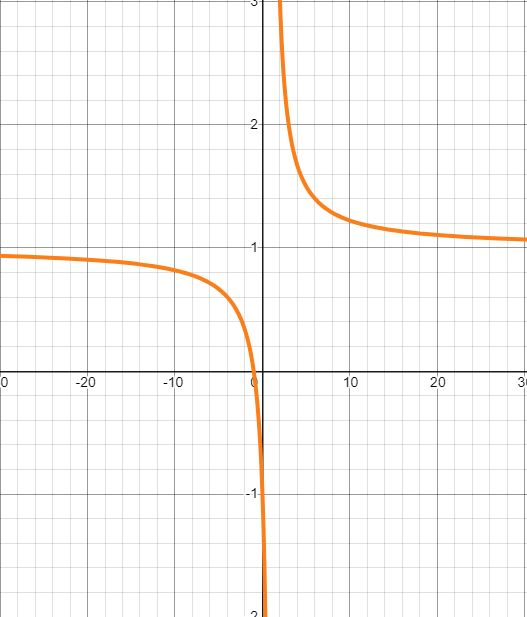
\includegraphics[width=10cm, height=6cm]{Four.JPG}
          \\
          \\
        }
      
      \item $\lim\limits_{x \to \infty} \dfrac{3x^2+1}{4x^3+x}$. 

        \textcolor{hwColor}{
          \\
          $
            \lim\limits_{x \to \infty} \dfrac{3x^2+1}{4x^3+x}
            =\lim\limits_{x \to \infty} \dfrac{\dfrac{3}{x}+\dfrac{1}{x^3}}{4+\dfrac{1}{x^2}}
            =\dfrac{\lim\limits_{x \to \infty} \left(\dfrac{3}{x}+\dfrac{1}{x^3}\right)}{\lim\limits_{x \to \infty} \left(4+\dfrac{1}{x^2}\right)}
            =\dfrac{\lim\limits_{x \to \infty} \dfrac{3}{x}+\lim\limits_{x \to \infty} \dfrac{1}{x^3}}{\lim\limits_{x \to \infty} 4+ \lim\limits_{x \to \infty}\dfrac{1}{x^2}}
            =\dfrac{0+0}{4+0}
            \\
            \\
            \\
            \therefore ~~~~ \lim\limits_{x \to \infty} \dfrac{3x^2+1}{4x^3+x}=0 ~~~~ \checkmark
            \\
          $
          \\
          \\
          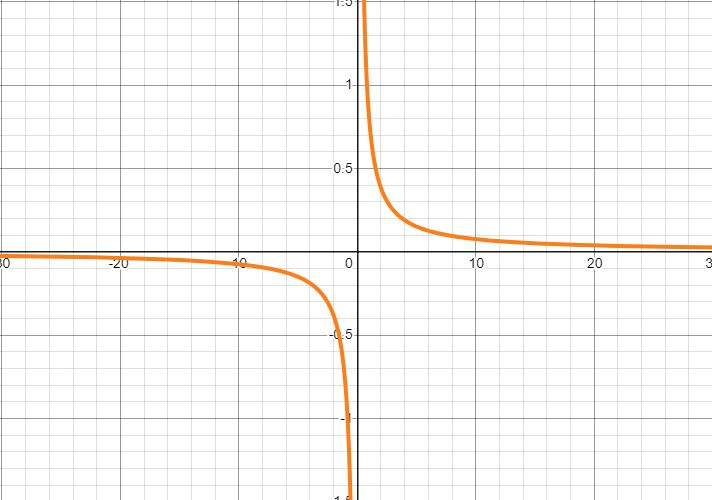
\includegraphics[width=10cm, height=6cm]{Three.JPG}
          \\
          \\
        }

    \end{itemize}

    \item Evaluate each of the following integrals. 
    \begin{itemize}
      \item $\bigints \dfrac{1}{x^3} dx$.

        \textcolor{hwColor}{
          \\
          $
            \bigints \dfrac{1}{x^3} dx
            =-\dfrac{x^{-2}}{2}
            \\
            \\
            \\
            \therefore ~~~~ \bigints \dfrac{1}{x^3} dx=-\dfrac{1}{2x^2}+C ~~~~ \checkmark
            \\
          $
        }

      \item $\bigints \dfrac{1}{3t+2} dt$.

        \textcolor{hwColor}{
          \\
          $
            u=3t+2, ~~~~ du=3dt
            \\
            \\
            \bigints \dfrac{1}{3t+2} dt
            =\bigints \dfrac{1}{u} \dfrac{du}{3}
            =\dfrac{1}{3} ln|u|
            =\dfrac{1}{3} ln|3t+2|
            \\
            \\
            \\
            \therefore ~~~~ \bigints \dfrac{1}{3t+2} dt=\dfrac{1}{3} ln|3t+2|+C ~~~~ \checkmark
            \\
          $
        }

      \item $\bigints e^{-3t} dt$.

        \textcolor{hwColor}{
          \\
          $
            u=-3t, ~~~~ du=-3dt
            \\
            \\
            \bigints e^{-3t} dt=\bigints e^u \dfrac{-du}{3}
            =-\dfrac{1}{3} e^u
            =-\dfrac{1}{3} e^{-3t}
            \\
            \\
            \\
            \therefore ~~~~ \bigints e^{-3t} dt=-\dfrac{1}{3} e^{-3t}+C ~~~~ \checkmark
            \\
          $
        }

      \item $\bigints t e^{-t} dt$.

        \textcolor{hwColor}{
          \\
          $
            \begin{cases}
              u=t
              \\
              dv=e^{-t} dt
            \end{cases} \Longrightarrow \begin{cases}
              du=dt 
              \\
              v=-e^{-t}
            \end{cases}
            \\
            \\
            \\
            \bigints t e^{-t} dt=t \left(-e^{-t}\right)-\bigints \left(-e^{-t}\right) dt
            =-t e^{-t}+\bigints \left(e^{-t}\right) dt
            =-te^{-t}-e^{-t}
            =-e^{-t} \left(-t-1\right)
            \\
            \\
            \\
            \therefore ~~~~ \bigints t e^{-t} dt=-e^{-t} \left(t+1\right)+C ~~~~ \checkmark
            \\
          $
        }

      \item $\bigints \dfrac{x}{x^2+1} dx$.

        \textcolor{hwColor}{
          \\
          $
            u=x^2+1, ~~~~ du=2xdx
            \\
            \\
            \bigints \dfrac{x}{x^2+1} dx=\bigints \dfrac{x}{u} \dfrac{du}{2x}
            =\dfrac{1}{2} \bigints\dfrac{1}{u} du
            =\dfrac{1}{2} ln|u|
            \\
            \\
            \\
            \therefore ~~~~ \bigints \dfrac{x}{x^2+1} dx=\dfrac{1}{2} ln|x^2+1|+C ~~~~ \checkmark
            \\
          $
        }

      \item $\bigints \dfrac{x^2+1}{x} dx$.

        \textcolor{hwColor}{
          \\
          $
            \bigints \dfrac{x^2+1}{x} dx
            =\bigints \left(x+\dfrac{1}{x}\right) dx
            =\bigints xdx+\bigints \dfrac{1}{x} dx
            =\dfrac{1}{2} x^2+ln|x|
            \\
            \\
            \\
            \therefore ~~~~ \bigints \dfrac{x^2+1}{x} dx=\dfrac{1}{2} x^2+ln|x|+C ~~~~ \checkmark
            \\
          $
        }

      \item $\bigints \dfrac{1}{x^2+1}dx$.

        \textcolor{hwColor}{
          \\
          $
            x=tan(\theta), ~~~~ dx=sec^2(\theta) d\theta
            \\
            \\
            \bigints \dfrac{1}{x^2+1^2}=\bigints \dfrac{1}{tan^2(\theta)+1} sec^2(\theta) d\theta
            =\bigints \dfrac{sec^2(\theta)}{sec^2(\theta)} d\theta
            =\bigints d\theta=\theta
            \\
            \\
            \\
            \therefore ~~~~ \bigints \dfrac{1}{x^2+1}dx=Arctan(x)+C ~~~~ \checkmark
            \\
          $
        }

      \item $\bigints\limits_{0}^{\dfrac{\pi}{4}} cos(2t) sin(2t) dt$.

        \textcolor{hwColor}{
          \\
          We know that $sin(\alpha) cos(\beta)=\dfrac{1}{2} \left[sin(\alpha+\beta)+sin(\alpha-\beta)\right]$.
          \\
          \\
          $
            \bigints cos(2t) sin(2t) dt=\bigints \dfrac{1}{2} \left[sin(2t+2t)+sin(2t-2t)\right] dt
            =\bigints \dfrac{1}{2} sin(4t) dt
            \\
            \\
            u=4t, ~~~~ du=4dt
            \\
            \\
            \bigints \dfrac{1}{2} sin(u) \dfrac{1}{4} dt=\dfrac{1}{8} \bigints sin(u) du
            =-\dfrac{1}{8} cos(u)
            =-\dfrac{1}{8} cos(4t)
            \\
            \\
            \\
            \bigints\limits_{0}^{\dfrac{\pi}{4}} cos(2t) sin(2t) dt
            =\left[-\dfrac{1}{8} cos(4t)\right]_{0}^{\dfrac{\pi}{4}}
            =\left[-\dfrac{1}{8} cos(4\dfrac{\pi}{4})\right]-\left[-\dfrac{1}{8} cos(4(0)))\right]
            \\
            \\
            \\
            \therefore ~~~~ \bigints\limits_{0}^{\dfrac{\pi}{4}} cos(2t) sin(2t) dt=\dfrac{1}{4} ~~~~ \checkmark
          $
        }

      \item $\bigints\limits_{0}^{\dfrac{\pi}{4}} e^t cos(t) dt$.

        \textcolor{hwColor}{
          \\
          $
            \begin{cases}
              u=e^t
              \\
              dv=cos(t)
            \end{cases} \Longrightarrow \begin{cases}
              du=e^t dt 
              \\
              v=sin(t)
            \end{cases}
            \\
            \\
            \\
            \bigints e^t cos(t) dt=e^t sin(t)-\bigints sin(t) e^t dt ~~~~ (A)
            \\
            \\
            \begin{cases}
              u=e^t 
              \\
              dv=sin(t)
            \end{cases} \Longrightarrow \begin{cases}
              du=e^t dt 
              \\
              v=-cos(t)
            \end{cases}
            \\
            \\
            \\
            \bigints sin(t) e^t dt=e^t (-cos(t))- \bigints -cos(t) e^t dt
            =e^t (-cos(t))+ \bigints cos(t) e^t dt ~~~~ (B)
            \\
            \\
          $
          Plugging (B) into (A) we have:
          \\
          \\
          $
            \bigints e^t cos(t) dt=e^t sin(t)-\left[e^t (-cos(t))- \bigints -cos(t) e^t dt\right]
            =e^t sin(t)+e^t cos(t)-\bigints cos(t) e^t dt 
            \\
            \\
            \therefore ~~~~ \bigints e^t cos(t) dt=e^t sin(t)+e^t cos(t)-\bigints cos(t) e^t dt
            \\
            \\
            \\
            \therefore ~~~~ 2 \bigints e^t cos(t) dt=e^t sin(t)+e^t cos(t)
            \\
            \\
            \\
            \therefore ~~~~  \bigints e^t cos(t) dt=\dfrac{1}{2} \left[e^t sin(t)+e^t cos(t)\right]
            \\
            \\
            \\
            \therefore ~~~~ \bigints\limits_{0}^{\dfrac{\pi}{4}} e^t cos(t) dt=\dfrac{e^t}{2} \left[sin(t)+cos(t)\right]_{0}^{\dfrac{\pi}{4}}
            \\
            \\
            \\
            =\dfrac{e^{\dfrac{\pi}{4}}}{2} \left[sin(\dfrac{\pi}{4})+cos(\dfrac{\pi}{4})\right]
            -\dfrac{e^0}{2} \left[sin(0)+cos(0)\right]
            \\
            \\
            \\
            =\dfrac{e^{\dfrac{\pi}{4}}}{2} \left[\dfrac{\sqrt{2}}{2}+\dfrac{\sqrt{2}}{2}\right]
            -\dfrac{1}{2} \left[0+1\right]
            \\
            \\
            \\
            \therefore ~~~~ \bigints\limits_{0}^{\dfrac{\pi}{4}} e^t cos(t) dt=\dfrac{\sqrt{2} e^{\dfrac{\pi}{4}}-1}{2}=\dfrac{e^{\dfrac{\pi}{4}}}{\sqrt{2}}-\dfrac{1}{2} ~~~~ \checkmark
          $
        }

      \item $\bigints\limits_{0}^{\dfrac{\pi}{4}} tan(x) dx$.

        \textcolor{hwColor}{
          \\
          $
            \bigints tan(x) dx=\bigints \dfrac{sin(x)}{cos(x)} dx
            \\
            \\
            u=cos(x), ~~~~ du=-sin(x)dx
            \\
            \\
            \bigints \dfrac{sin(x)}{cos(x)} dx=\bigints \dfrac{sin(x)}{u} \dfrac{-du}{sin(x)}
            =-\bigints \dfrac{1}{u} du
            =-ln|u|=-ln|cos(x)|+C
            \\
            \\
            \\
            \therefore ~~~~ \bigints\limits_{0}^{\dfrac{\pi}{4}} tan(x) dx=ln|cos(x)|_{0}^{\dfrac{\pi}{4}}
            =-ln|cos(\dfrac{\pi}{4})|+ln|cos(0)|
            =-ln|\dfrac{\sqrt{2}}{2}|+ln|1|
            \\
            \\
            \\
            \therefore ~~~~ \bigints\limits_{0}^{\dfrac{\pi}{4}} tan(x) dx=ln|cos(x)|_{0}^{\dfrac{\pi}{4}}=\dfrac{1}{2} ln(2) ~~~~ \checkmark
          $
        }

      \item $\bigints \dfrac{x}{\sqrt{x^2+1}} dx$.

        \textcolor{hwColor}{
          \\
          $
            u=x^2+1, ~~~~ du=2x dx
            \\
            \\
            \bigints \dfrac{x}{\sqrt{x^2+1}} dx=\bigints \dfrac{x}{\sqrt{u}} \dfrac{du}{2x}
            =\bigints \dfrac{1}{2\sqrt{u}} du
            =\dfrac{1}{2} \bigints u^{-\dfrac{1}{2}} du
            =\dfrac{1}{2} \dfrac{u^{-\dfrac{1}{2}+1}}{-\dfrac{1}{2}+1}
            \\
            \\
            =\dfrac{1}{2} \dfrac{u^{\dfrac{1}{2}}}{\dfrac{1}{2}}
            =\sqrt{u}
            =\sqrt{x^2+1}
            \\
            \\
            \\
            \therefore ~~~~ \bigints \dfrac{x}{\sqrt{x^2+1}} dx=\sqrt{x^2+1}+C ~~~~ \checkmark
            \\
          $
        }
        
    \end{itemize}


  \end{enumerate}

\end{document}
